
% Copyright (c) 2015 - 2020 Mario Mlačak, mmlacak@gmail.com
% Public Domain work, under CC0 1.0 Universal Public Domain Dedication. See LICENSING, COPYING files for details.

% Age of Aquarius chapter =============================================
\chapter*{Age of Aquarius}
\addcontentsline{toc}{chapter}{Age of Aquarius}
\label{ch:Age of Aquarius}

\begin{flushright}
\parbox{0.8\textwidth}{
\emph{The human mind is inspired enough when it comes to inventing
horrors; it is when it tries to invent a Heaven that it shows itself
cloddish.\newline
\hspace*{\fill}{\textasciitilde{} Evelyn Waugh} } }
\end{flushright}

\noindent
Age of Aquarius is chess variant which is played on 14 $\times$ 14 board,
with light yellow and light green fields and light tan-gold and
dark green pieces. A new piece is introduced, Unicorn.

\clearpage % ..........................................................
% Unicorn *************************************************************

\section*{Unicorn}
\addcontentsline{toc}{section}{Unicorn}
\label{sec:Age of Aquarius/Unicorn}

\noindent
\begin{wrapfigure}[5]{l}{0.4\textwidth}
\centering
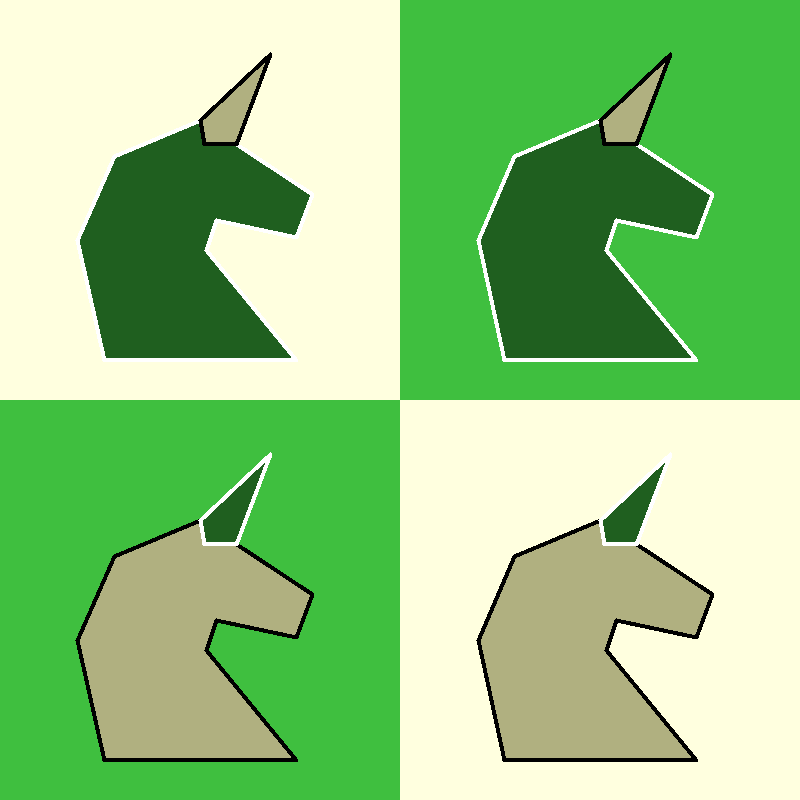
\includegraphics[width=0.4\textwidth, keepaspectratio=true]{pieces/09_unicorn.png}
\caption{Unicorn}
\label{fig:09_unicorn}
\end{wrapfigure}
Unicorn is a piece similar to Knight, only it can jump longer on
opposite color fields. Just as Knight, Unicorn is not obstructed
by any piece in its surroundings.

\vspace{6.0\baselineskip}
\subsection*{Movement}
\addcontentsline{toc}{subsection}{Movement}
\label{sec:Age of Aquarius/Unicorn/Movement}

\noindent
\begin{wrapfigure}{l}{0.4\textwidth}
\centering
\includegraphics[width=0.4\textwidth, keepaspectratio=true]{examples/08_aoa/scn_aoa_01_unicorn_same_color.png}
\caption{Unicorn short jump}
\label{fig:scn_aoa_01_unicorn_same_color}
\end{wrapfigure}
On fields with the same color as Unicorn, it can move exactly the
same way Knight does.

\clearpage % ..........................................................

\noindent
\begin{figure}[!h]
\includegraphics[width=1.0\textwidth, keepaspectratio=true]{examples/08_aoa/scn_aoa_02_unicorn_opposite_color.png}
\caption{Unicorn long jump}
\label{fig:scn_aoa_02_unicorn_opposite_color}
\end{figure}

On fields in opposite color, Unicorn can jump much longer. Again, just as
Knight, Unicorn is not hampered by surrounding pieces. Own pieces on marked
step-fields would prevent Unicorn to move. The same marked fields are also
capture-fields, opponent's pieces on them could be captured.

For comparison, Knight's step-fields are also numbered (gray).

% ************************************************************* Unicorn
\clearpage % ..........................................................
% Promotion ***********************************************************

\section*{Promotion}
\addcontentsline{toc}{section}{Promotion}
\label{sec:Age of Aquarius/Promotion}

In all variants prior to this one promotion was forced, Pawn had to be
promoted immediately upon reaching opposite end of chessboard (or when
\hyperref[sec:Mayan Ascendancy/Pyramid/Promotion]{reached by own Pyramid} on
\hyperref[sec:Definitions/Chessboard sides, navigation]{opponent's side of the board}).
Promotion otherwise is identical to one in Classical Chess, which is
described in details here:\newline
\href{https://en.wikipedia.org/wiki/Promotion\_(chess)}{https://en.wikipedia.org/wiki/Promotion\_(chess)}.

In this variant promotion is not forced, Pawn does not have to be promoted
immediately, or at all. Pawn can be promoted later in a game, if it hasn't
moved between being tagged for promotion and actual promotion itself. Thus,
promotion can take place only on a field at which Pawn has been tagged for
promotion.

Tag is a link between a piece and a field at which it stands, representing
delayed opportunity. So, if tagged Pawn moves before actual promotion, the
Pawn loses its tag, and cannot be promoted anymore. Field at which Pawn has
been tagged for promotion does not hold tag, and does not grant ability to
promote to any other Pawn passing over it.

If Pawn tagged for promotion gets captured or converted, that opportunity
has been lost. Neither converted Pawn (now opponent's), nor any other Pawn
(own or opponent's), can be promoted on the field at which Pawn has been
converted.

Delayed promotion is a complete move, it can contain only promotion of one
Pawn and nothing else.

\clearpage % ..........................................................

\noindent
\begin{figure}[h]
\includegraphics[width=1.0\textwidth, keepaspectratio=true]{examples/08_aoa/scn_aoa_03_delayed_promo_init.png}
\caption{Promotion start}
\label{fig:scn_aoa_03_delayed_promo_init}
\end{figure}

Here, light player is about to tag Pawn 2 for promotion, using Pyramid
activated by Bishop. Note, Pawn 3 is not yet eligible for promotion, as it's
still on own side of chessboard.

\clearpage % ..........................................................

\noindent
\begin{figure}[h]
\includegraphics[width=1.0\textwidth, keepaspectratio=true]{examples/08_aoa/scn_aoa_04_delayed_promo_pawn_2_tagged.png}
\caption{Pawn 2 tagged for promotion}
\label{fig:scn_aoa_04_delayed_promo_pawn_2_tagged}
\end{figure}

To speed things up, next images show dark player's response (grey arrow),
and light player's plan for next move (green arrow). Each depicted position
is after dark player's move, but before light player's move.

Here, dark Unicorn is attacking tagged Pawn 2. Pawn 2 is to move next.

\clearpage % ..........................................................

\noindent
\begin{figure}[h]
\includegraphics[width=1.0\textwidth, keepaspectratio=true]{examples/08_aoa/scn_aoa_05_delayed_promo_pawn_2_moved.png}
\caption{Pawn 1 about to get promotion}
\label{fig:scn_aoa_05_delayed_promo_pawn_2_moved}
\end{figure}

Dark Unicorn closed in, attacking both Pawn 2 and Bishop. Since Pawn 2 moved
away from field P at which it was tagged for promotion, that opportunity has
been lost, and can't be recovered. Label P on a field just marks where Pawn 2
was tagged for promotion. Field P isn't special in any way, it won't make e.g.
Pawn 3 tagged for promotion when reached.

Light Pawn 1 is about to go next.

\clearpage % ..........................................................

\noindent
\begin{figure}[h]
\includegraphics[width=1.0\textwidth, keepaspectratio=true]{examples/08_aoa/scn_aoa_06_delayed_promo_pawn_1_tagged.png}
\caption{Pawn 1 tagged for promotion}
\label{fig:scn_aoa_06_delayed_promo_pawn_1_tagged}
\end{figure}

Light Pawn 1 is now tagged for promotion, and is to be promoted later.
Dark Unicorn closed in again, capturing light Bishop.

Light Pawn 2 is about to go next.

\clearpage % ..........................................................

\noindent
\begin{figure}[h]
\includegraphics[width=1.0\textwidth, keepaspectratio=true]{examples/08_aoa/scn_aoa_07_delayed_promo_pawn_1_promoted.png}
\caption{Pawn 1 promoted}
\label{fig:scn_aoa_07_delayed_promo_pawn_1_promoted}
\end{figure}

Dark Unicorn captures light Pawn 2.

Light Pawn 1 is promoted to Queen.

\clearpage % ..........................................................
% Converting tagged Pawn ----------------------------------------------

\subsection*{Converting tagged Pawn}
\addcontentsline{toc}{subsection}{Converting tagged Pawn}
\label{sec:Age of Aquarius/Promotion/Converting tagged Pawn}

\noindent
\begin{figure}[h]
\includegraphics[width=1.0\textwidth, keepaspectratio=true]{examples/08_aoa/scn_aoa_08_converting_tagged_pawn_init.png}
\caption{Tagging Pawn for promotion}
\label{fig:scn_aoa_08_converting_tagged_pawn_init}
\end{figure}

Pawn tagged for promotion after being converted loses its tag, and with it opportunity to promote.

Here, light Pawn would be tagged for promotion, after light player completes its move.

\clearpage % ..........................................................

\noindent
\begin{figure}[h]
\includegraphics[width=1.0\textwidth, keepaspectratio=true]{examples/08_aoa/scn_aoa_09_converting_tagged_pawn_end.png}
\caption{Converting tagged Pawn}
\label{fig:scn_aoa_09_converting_tagged_pawn_end}
\end{figure}

Opponent pieces (except King) can be \hyperref[sec:Mayan Ascendancy/Pyramid/Conversion]{converted into own pieces}, on own side of chessboard.
So, Pawns tagged for promotion are also valid objects of conversion.

Here, light Pawn tagged for promotion would be converted, and its tag would be invalidated, after dark player completes its move.

\clearpage % ..........................................................

\noindent
\begin{figure}[h]
\includegraphics[width=1.0\textwidth, keepaspectratio=true]{examples/08_aoa/scn_aoa_10_tagged_pawn_converted.png}
\caption{Tagged Pawn converted}
\label{fig:scn_aoa_10_tagged_pawn_converted}
\end{figure}

Tag for promotion is a link between a piece and field at which it's situated.

Now that light Pawn tagged for promotion is gone, that link is broken.
To be able to promote, a new tag has to be established between converted dark Pawn and its location, on light side of chessboard.

% ---------------------------------------------- Converting tagged Pawn
% *********************************************************** Promotion
\clearpage % ..........................................................

\section*{Rush, en passant}
\addcontentsline{toc}{section}{Rush, en passant}
\label{sec:Age of Aquarius/Rush, en passant}

\noindent
\begin{wrapfigure}{l}{0.4\textwidth}
\centering
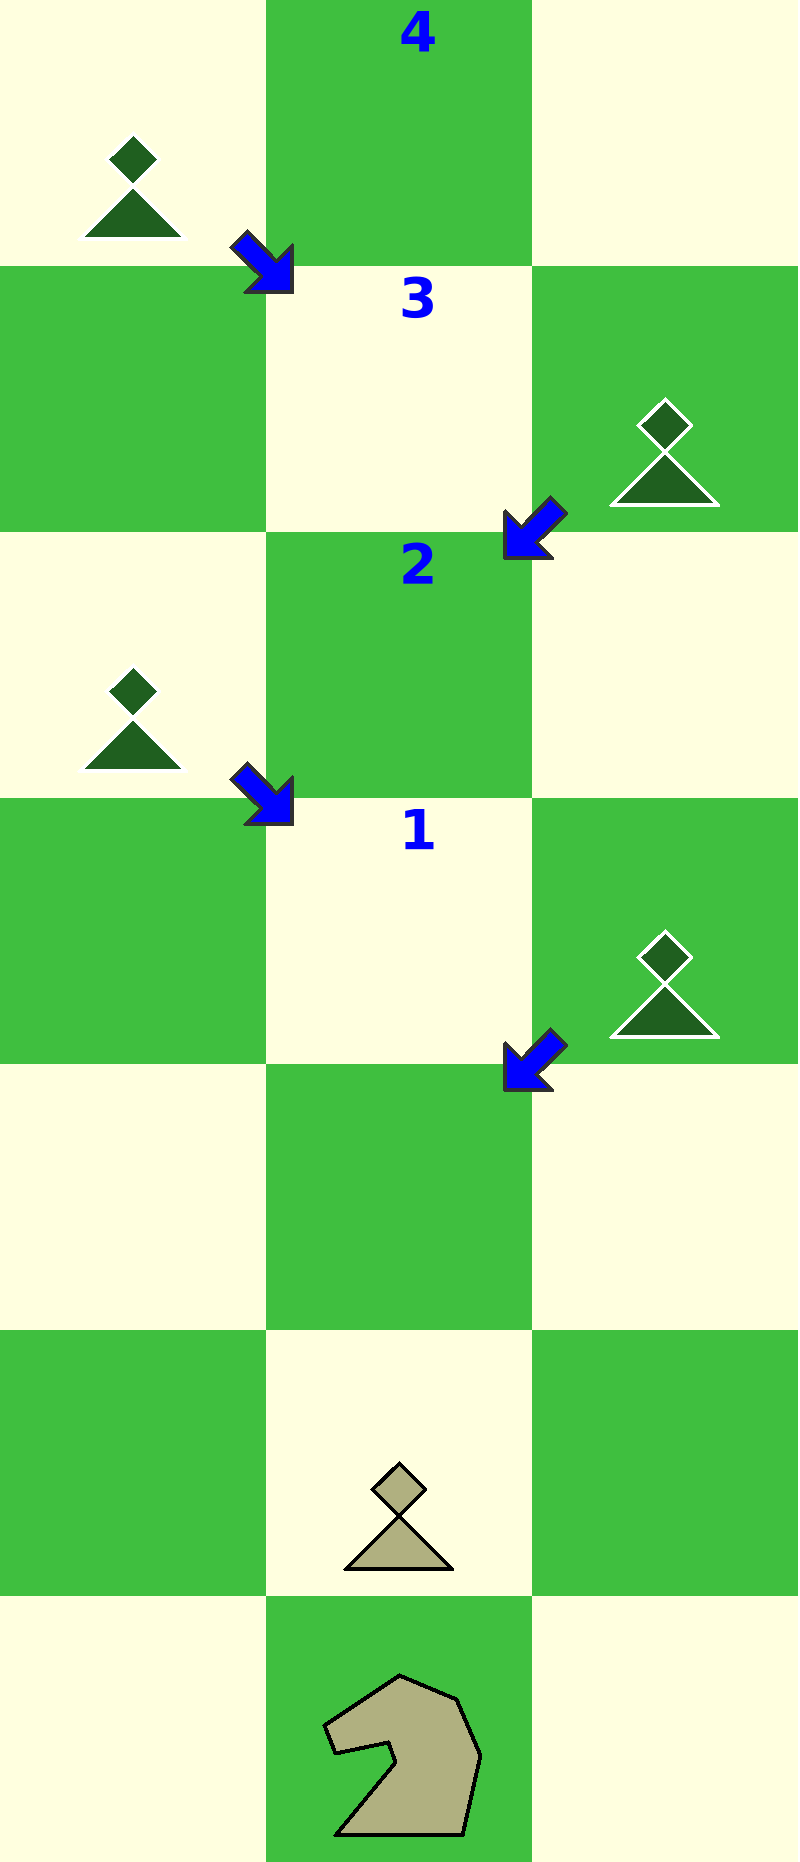
\includegraphics[width=0.235714286\textwidth, keepaspectratio=true]{en_passants/08_age_of_aquarius_en_passant.png}
\caption{En passant}
\label{fig:08_age_of_aquarius_en_passant}
\end{wrapfigure}
Rush and en passant are identical to those in Classic Chess, only difference
is that Pawn can now move longer on initial turn, up to 5 fields in this
variant.

\clearpage % ..........................................................

\section*{Castling}
\addcontentsline{toc}{section}{Castling}
\label{sec:Age of Aquarius/Castling}

Castling is the same as in Classical Chess, only difference is that King can move 2, 3, 4 or 5 fields across.
All other constraints from Classical Chess still applies.

\noindent
\begin{figure}[!h]
\includegraphics[width=1.0\textwidth, keepaspectratio=true]{castlings/08_aoa/age_of_aquarius_castling.png}
\caption{Castling}
\label{fig:age_of_aquarius_castling}
\end{figure}

In example above, all valid King's castling moves are numbered.

\noindent
\begin{figure}[!h]
\includegraphics[width=1.0\textwidth, keepaspectratio=true]{castlings/08_aoa/age_of_aquarius_castling_left_04.png}
\caption{Castling long left}
\label{fig:age_of_aquarius_castling_left_04}
\end{figure}

In this example King was castling long to the left. Initial King's position is marked with "K".
After castling is finished, left Rook ends up on the field immediately right to the King.

\clearpage % ..........................................................

\section*{Initial setup}
\addcontentsline{toc}{section}{Initial setup}
\label{sec:Age of Aquarius/Initial setup}

Compared to initial setup of Mayan Ascendancy, Unicorn is inserted between Pyramid and Knight
symmetrically, on both sides of chessboard. This can be seen in the image below:

\noindent
\begin{figure}[h]
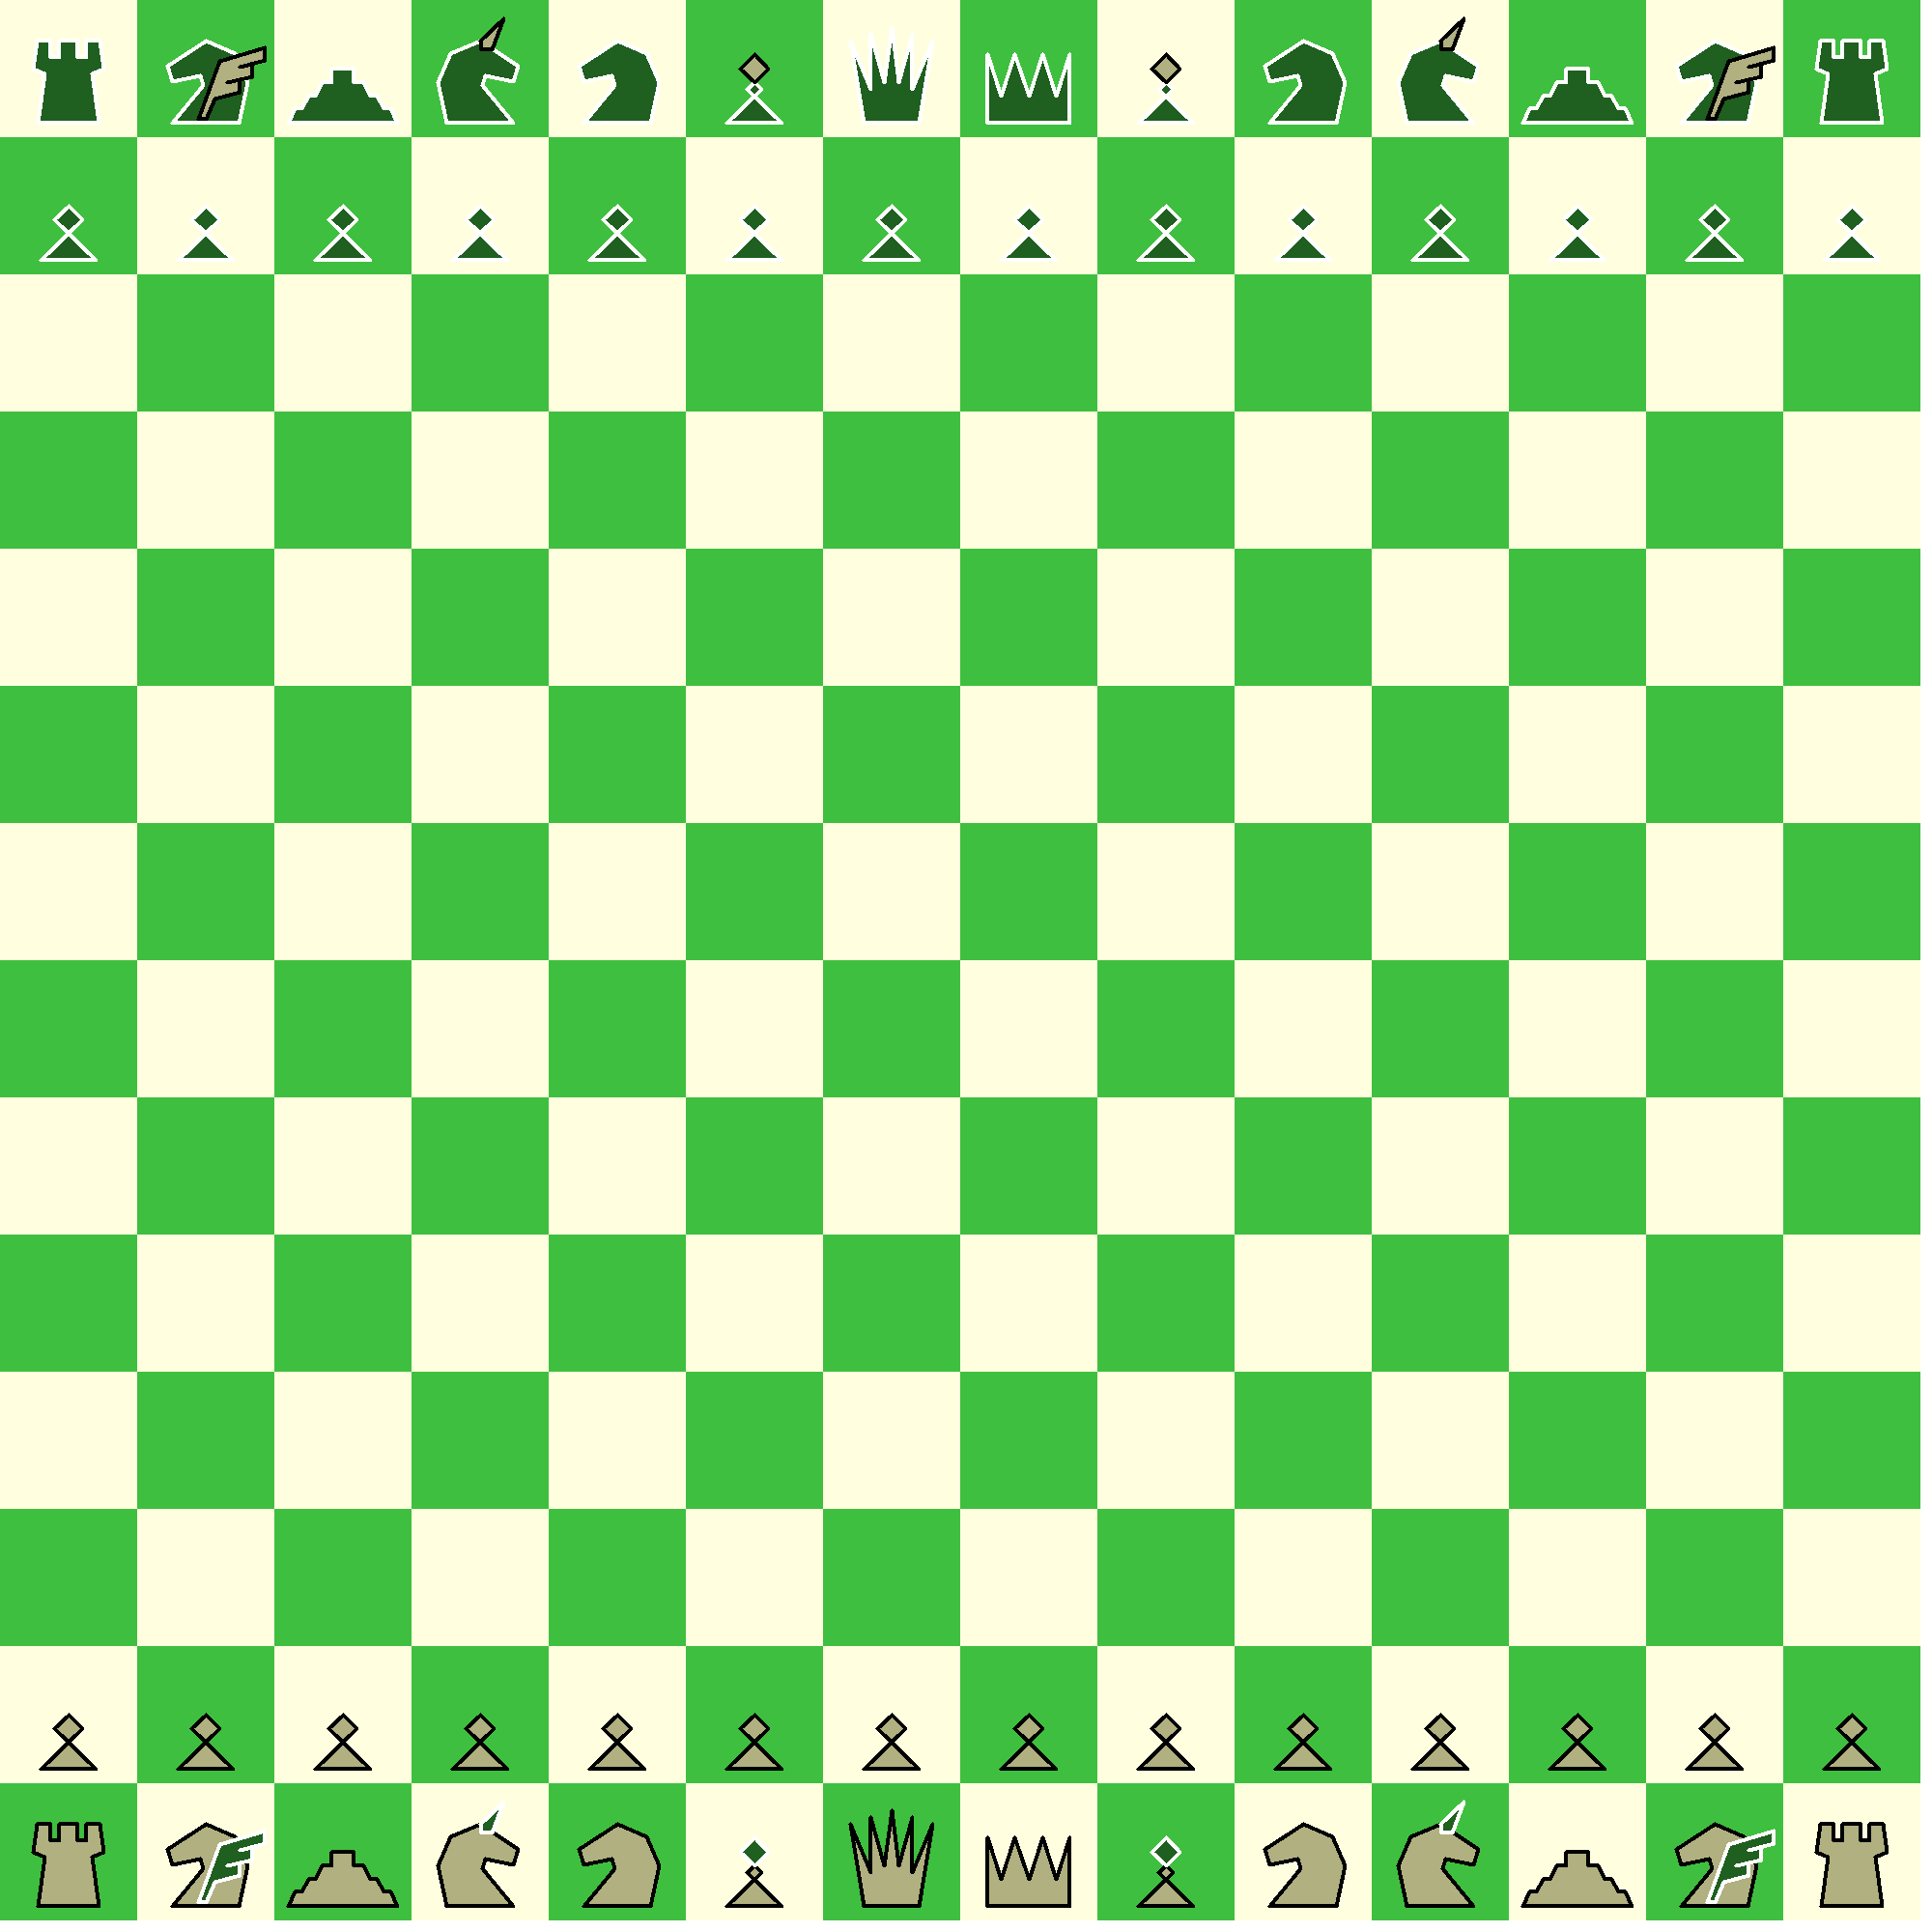
\includegraphics[width=1.0\textwidth, keepaspectratio=true]{boards/08_age_of_aquarius.png}
\caption{Age of Aquarius board}
\label{fig:08_age_of_aquarius}
\end{figure}

\clearpage % ..........................................................
% ============================================= Age of Aquarius chapter
